\section{Next-to-leading order and renormalization}
We have now regularized the divergences, so they can be handled in a well-defined way.
However, they are still there.
To get rid of them, we need to use renormalization.
The power counting scheme used when constructing the Effective Lagrangians ensures that all terms in $\Ell_{2n}$ is of order $p^{2n}$ in the pion momenta.\footnote{Remember that the bare pion mass $\bar m = B_0(m_u + m_d)$ is considered to be of order $p^2$.}
The tree level free energy from $\Ell_{2n}$ is thus of order $p^{2n}$.
The n-loop correction to the tree level result is then suppressed by $p^{2n}$~\cite{Gasser-Leutwyler:chiral,WeinbergPhenom}.
Our one-loop calculation using $\Ell_2$ therefore contains divergences of order $p^{4}$. 
Since $\Ell_4$ is, by construction, the most general possible Lagrangian at order $p^4$, it contains coupling constants which can be renormalized to absorb all these divergences.

The renormalized coupling constants in $\Ell_2$ have been calculated for $\mu_I = 0$~\cite{Gasser-Leutwyler:chiral}.
They are independent of $\mu_I$, and we can therefore use them in this calculation.
The renormalized coupling constants in the $\overline{\mathrm{MS}}$-scheme are related to the bare couplings through
\begin{align}
    l_i 
    & = 
    l_i^r 
    - \mu^{-2\epsilon}\frac{1}{2} \frac{\gamma_i }{(4 \pi)^2} 
    \left(\frac{1}{\epsilon} + 1 \right),
    \quad \quad
    i \in \{1, ... 7\} 
    \\
    h_i 
    & = 
    h_i^r
    - \mu^{-2\epsilon} \frac{1}{2}  \frac{\delta_i }{(4 \pi)^2} 
    \left(\frac{1}{\epsilon} + 1 \right), 
    \quad \quad
    i \in \{1, ... 3\}.
\end{align}
Here, $\gamma_i$ and $\delta_i$ are numerical constants that are used to match the divergences.
The relevant terms are\footnote{Some authors~\cite{Andersen:two-flavor-chpt,GERBER1989387} instead use $h_1' = h_1 - l_4$, with a corresponding $\delta_1' = \delta_1 - \gamma_1 = 0$.}
\begin{gather}
    \gamma_1 = \frac{1}{3}, \quad
    \gamma_2 = \frac{2}{3}, \quad
    \gamma_3 = - \frac{1}{2}, \quad
    \gamma_4 = 2, \\
    \delta_1 = 2, \quad
    \delta_3 = 0.
\end{gather}
The bare coupling constants, though infinite, are independent of our renormalization scale $\mu$.
From this we obtain the renormalization group equations for the running coupling constants,
\begin{equation}
    \mu \diff{l_i^r}{\mu } = - \mu^{-2\epsilon} \frac{\gamma_i }{(4 \pi)^2}, \quad
    \mu \diff{h_i^r}{\mu } = -  \mu^{-2\epsilon}\frac{\delta_i}{(4 \pi)^2}.
\end{equation}
These have the general solutions
\begin{equation}
    l_i^r 
    = \frac{1}{2} \mu^{-2\epsilon} \frac{\gamma_i}{(4 \pi)^2} 
    \left( \bar l_i - \ln{\frac{\mu^2}{M^2}} \right),
    \quad
    h_i^r 
    = \frac{1}{2} \mu^{-2\epsilon} \frac{\gamma_i}{(4 \pi)^2} 
    \left( \bar h_i - \ln{\frac{\mu^2}{M^2}} \right),
\end{equation}
where $\bar l_i$ and $\bar h_i$ are the values of the coupling constants (times a constant) measured at the energy $M$.
This only applies if the numerical constants $\gamma_i$/$\delta_i$ are non-zero.
If they are zero, then the renormalized constant is not running, and instead equal to its measured value at all energies.
The bare couplings are thus given by
\begin{equation}
    \label{bare couplings as functions of measured values}
    l_i = \mu^{-2\epsilon} \frac{1}{2} \frac{\gamma_i}{(4 \pi)^2}
    \left(
        \bar l_i -1- \frac{1}{\epsilon} - \ln\frac{\mu^2}{M^2}
    \right), 
    \quad
    h_i = \mu^{-2\epsilon} \frac{1}{2} \frac{\delta_i}{(4 \pi)^2}
    \left(
        \bar h_i - 1 - \frac{1}{\epsilon} - \ln\frac{\mu^2}{M^2}
    \right)
\end{equation}
The next-to-leading contribution to the free energy at tree-level is $\Ef_4^{0} = - \Ell_4^{(0)}$, which is given by \cref{NLO-L0}.
When substituting \autoref{bare couplings as functions of measured values} into the bare couplings, we get
\begin{align*}
    \Ef^{(0)}_4
    & = 
    - (l_1 + l_2)\mu_I^4 \sin^4{\alpha}
    - (l_3 + l_4)\bar m^4 \cos^2{\alpha}
    - l_4 \bar m^2 \mu_I{}^2 \cos{\alpha} \sin^2{\alpha}
    -(h_1- l_4) \bar m^4
    - h_3 \Delta m^4
    \\
    & = 
    - \mu^{-2 \epsilon} \frac{1}{2} \frac{1}{(4 \pi)^2}
    \bigg[
        \frac{1}{3}
        \left( 
            \bar l_1 + 2 \bar l_2 - 3
        \right) \mu_I^4 \sin^4 \alpha
        +
        \frac{1}{2}
        \left(
            - \bar l_3 + 4 \bar l_4 - 3
        \right) \bar m^4 \cos^2\alpha
        \\
        & \quad \quad \quad \quad \quad
        + 2 \left(\bar l_4 - 1\right)
        \bar m^2 \mu_I^2 \cos\alpha \sin^2 \alpha
        + 2 (\bar l_4 - \bar h_1) \bar m^4
        + \bar h_3 \Delta m^4
        \\
        & \quad \quad \quad \quad \quad
        - 
        \left(\frac{1}{\epsilon} + \ln \frac{\mu^2}{M^2}\right) 
        \left(
            \mu_I^4\sin^4\alpha + \frac{3}{2} \bar m^4 \cos^2 \alpha
            + 2 \bar m^2 \mu_I^2 \cos\alpha \sin^2 \alpha
        \right) 
    \bigg] 
\end{align*}
Notice that the term proportional to $\epsilon^{-1}$ cancel exactly with the divergent term from $\Ef^{(2)}$, as we expected.
Adding all the contribution to the free energy density, and taking the limit $\epsilon \rightarrow 0$, we get the next-to-leading order free energy,
\begin{align}
    \nonumber
    \Ef_{\mathrm{NLO}} &=
    - f^2 \left(\bar m^2 \cos \alpha + \frac{1}{2}\mu_I^2 \sin^2 \alpha\right)
    + \Ef^{(1)}_{\mathrm{fin}, \pi_\pm}
    - \frac{1}{2}\frac{1}{(4 \pi)^2}
    \bigg[
        \frac{1}{3}
        \left( 
            \bar l_1 + 2 \bar l_2 + \frac{3}{2} + 3 \ln \frac{M^2}{m_3^2}
        \right) \mu_I^4 \sin^4 \alpha
        \\ %\nonumber
        &
        +
        \frac{1}{2}
        \left(
            - \bar l_3 + 4 \bar l_4 + \frac{3}{2} + 2\ln \frac{M^2}{m_3^2}
            + \ln \frac{M^2}{\tilde m^2_2}
        \right) \bar m^4 \cos^2\alpha 
        + 2 \left(\bar l_4 - \frac{1}{2} + \ln \frac{M^2}{m_3^2}\right)
        \bar m^2 \mu_I^2 \cos\alpha \sin^2 \alpha
        \label{NLO free energy}
        % \\
        % & 
        % + 2 (\bar l_4 - \bar h_1) \bar m^2
        % + \bar h_3 \Delta m^2
    \bigg].
\end{align}
We have dropped the terms proportional to $\bar l_4 - \bar h_1$ and $\bar h_3$, as they only add an unobservable constant value to the free energy.



\subsection*{Parameters, and keeping the expansion consistent}
The coupling constants are free parameters, and can therefore not be calculated from first principles, but must be measured.
The values for the pion mass and pion decay constants are (HVORFOR?)
\begin{equation}
    m_\pi = 131 \, \mathrm{MeV}, \quad f_\pi = \frac{1}{\sqrt 2} 128 \, \mathrm{MeV}.
\end{equation}
This is the physical mass, $m_\pi$, is defined as the pole of the propagator and thus the zero of the inverse propagator,
\begin{equation}
    D^{-1}(p^2 = m_\pi^2) = 0.
\end{equation}
This relates it to the which relates it to the bare mass $\bar m$.
We found, in \cref{m1}, that $m_\pi^2 = m_3^2(\mu_I = 0) = \bar m^2$ to leading order.
Similarly, $f_\pi = f$ to leading order.
However, in any NLO results we need $\bar m^2$ and $f$ to NLO.
This is given by~\cite{Gasser-Leutwyler:chiral}
\begin{align}
    \label{equation bare mass}
    m_\pi^2 & = \bar m^2 + \frac{\bar l_3}{2 (4\pi)^2} \frac{\bar m^4}{f^2}, \\
    \label{equation bare decay constant}
    f_\pi^2 & = f^2 + \frac{2\bar l_4}{(4\pi)^2} \frac{\bar m^2}{f^2}
\end{align}
All results in this text are given in units of $m_\pi$.

\begin{table}[h]
    \centering
    \caption{The measured values and corresponding uncertainties of the relevant coupling constants.}
    \begin{tabular}{c c c c}
        \hline \hline
        & value & uncertainty & source \\
        \hline \\[-1em]
        $\bar l_1$ & -0.4   & \pm 0.6   & \cite{pipi_scattering}    \\
        $\bar l_2$ & 4.3    & \pm 0.1   & \cite{pipi_scattering}    \\
        $\bar l_3$ & 2.9    & \pm 2.4   & \cite{Gasser-Leutwyler:chiral} \\    
        $\bar l_4$ & 4.4    & \pm 0.2   & \cite{pipi_scattering}    \\
        \hline
    \end{tabular}
    \label{table:coupling constants}
\end{table}
The values for the coupling constants used in this text are given in \autoref{table:coupling constants}.
The constants $\bar l_1$, $\bar l_2$ and $\bar l_4$ are estimated using data from $\pi \pi$-scattering~\cite{pipi_scattering}, while $\bar l_3$ is estimated using three flavor chiral perturbation theory~\cite{Gasser-Leutwyler:chiral}.
These are the same values as those used in~\cite{Andersen:two-flavor-chpt}.
Together with \cref{equation bare mass,equation bare decay constant}, the NLO results for the bare mass and decay constant are
\begin{align}
    \label{NLO m}
    \bar m / m_\pi = 1.01136, \\
    \label{NLO f}
    f / m_\pi = 0.64835.
\end{align}

In \autoref{section: free energy at lowest order}, we found a relationship between $\alpha$ and $\mu_i$, using the lowest order estimate of $\Ef$, given in \cref{leading order minization}.
To calculate any thermodynamic quantities to leading order, at the tree-level, we must use this result.
When calculating higher order corrections to the free energy, we must make sure to calculate this and other relationship to the same order, consistently.
As we have seen earlier, when replacing the action by $S[\varphi] \rightarrow g^{-1}S[\varphi]$, the $L$-loop contribution is proportional to $g^{L-1}$.
The Weinberg's power counting scheme, when replace $p \rightarrow t p$, and $m \rightarrow t^2 m$, the n'th therm in the expansion is proportional to $t^{2n}$.
We can therefore expand the free energy as
\begin{equation}
    \Ef = t^2 g^{-1} \Ef_2^{(0)} + t^2 \Ef_2^{(1)} + t^4 g^{-1} \Ef_4^{(0)}
    + ...
\end{equation}
We consider terms where $m = L + n$ are the same to be of the same order.
This expansion can be written as
\begin{equation}
    \Ef = \sum_{m=0}^\infty \sum_{n+L=m} t^{2n} g^{L-1} \Ef_{2n}^{(L)}.
\end{equation}
If we now define
\begin{equation}
    \tilde \Ef_m = \sum_{n+L=m} t^{2n} g^{L-1} \Ef_{2n}^{(L)},
\end{equation}
then scale $t \rightarrow \sqrt{s} \, t$ and $g \rightarrow s g$, where $s$ is some real number, then $t^{2n}g^{L-1}$ scales as $s^{n+L-1} = s^{m-1}$.
We can therefore expand the free energy as
\begin{equation}
    s \Ef = \sum_{m= 0}^\infty \tilde \Ef_m \, s^{m}.
\end{equation}
The same expansion holds for all quantities we calculate from this theory.
Let $\alpha'$ be the solution to
\begin{equation}
    \diffp{\Ef}{\alpha} \bigg|_{\alpha=\alpha'} = 0
\end{equation}
to all orders.
We expand this solution in $s$,
\begin{equation}
    \alpha' = \alpha_0 + \alpha_1 s + \dots.
\end{equation}
Combining this, we get
\begin{align*}
    0 &
    = 
    \diffp{}{\alpha}
    \left[
        s^{-1}\tilde \Ef_0
        + 
        \tilde \Ef_1
        +
        \Oh[1]{s}
    \right]
    \bigg|_{\alpha=\alpha_0 + \alpha_1 s + \Oh{s}} 
    \\
    & = 
    s^{-1 }
    \left[
        \tilde \Ef_0'(\alpha_0)
        +
        (\alpha' - \alpha_0)
        \tilde \Ef_0''(\alpha_0)
        +
        \Oh[2]{s}
    \right]
    +
    \tilde\Ef_1'(\alpha_0)
    +
    \Oh[1]{s} \\
    &
    =
    s^{-1} \tilde\Ef_1'(\alpha_0)
    + s^{0}
    \left[
        \alpha_1
        \tilde \Ef_0''(\alpha_0)
        +
    \tilde\Ef_1'(\alpha_0)
    \right]
    +
    \Oh[1]{s}
\end{align*}
Here, the prime indicates partial derivatives with respect to $\alpha$.
This equality has to hold term for term.
After setting $s = g = t = 1$, we get
\begin{align*}
    \diffp{\tilde \Ef_0}{\alpha}\bigg|_{\alpha=\alpha_0} = 0, \quad
    \tilde \Ef_0 = \Ef_2^{(0)},
\end{align*}
which is what we have used as the leading-order result. 
The next to leading order result is
\begin{equation}
    \alpha_1 = - \frac{\tilde \Ef_1'(\alpha_0)}{{\tilde \Ef_0''(\alpha_0)}},
    \quad 
    \tilde \Ef_1 = \Ef_{4}^{(0)} + \Ef_{2}^{(1)}.
\end{equation}

The next to leading order results for the free energy and $\alpha'$ are
\begin{equation}
    \Ef_\mathrm{NLO} = \tilde \Ef_0 + \tilde \Ef_1, \quad
    \alpha_\mathrm{NLO} = \alpha_0 + \alpha_1.
\end{equation}
If we use this to result to obtain an NLO-version of the equation for $\alpha$, we get
\begin{equation}
    \Ef_\mathrm{NLO}'(\alpha_\mathrm{NLO})
    = \tilde \Ef_0'(\alpha_0) + \alpha_1 \tilde \Ef_0''(\alpha_0) + \dots
    + \tilde \Ef_1'(\alpha_0) + \dots,
\end{equation}
where the terms that are not included are beyond next-to-leading order.
Thus,
\begin{equation}
    \label{alpha nlo method 2}
    \diffp{\Ef_\mathrm{NLO}}{\alpha} \bigg|_{\alpha=\alpha'} = 0
\end{equation}
will give the correct answer to $\alpha'$ to next-to-leading order.

In \autoref{fig:alpha}, the leading order and next-to-leading order results for $\alpha'$ is shown.
The NLO result was calculated numerically using \cref{alpha nlo method 2}.
\begin{figure}
    \centering
    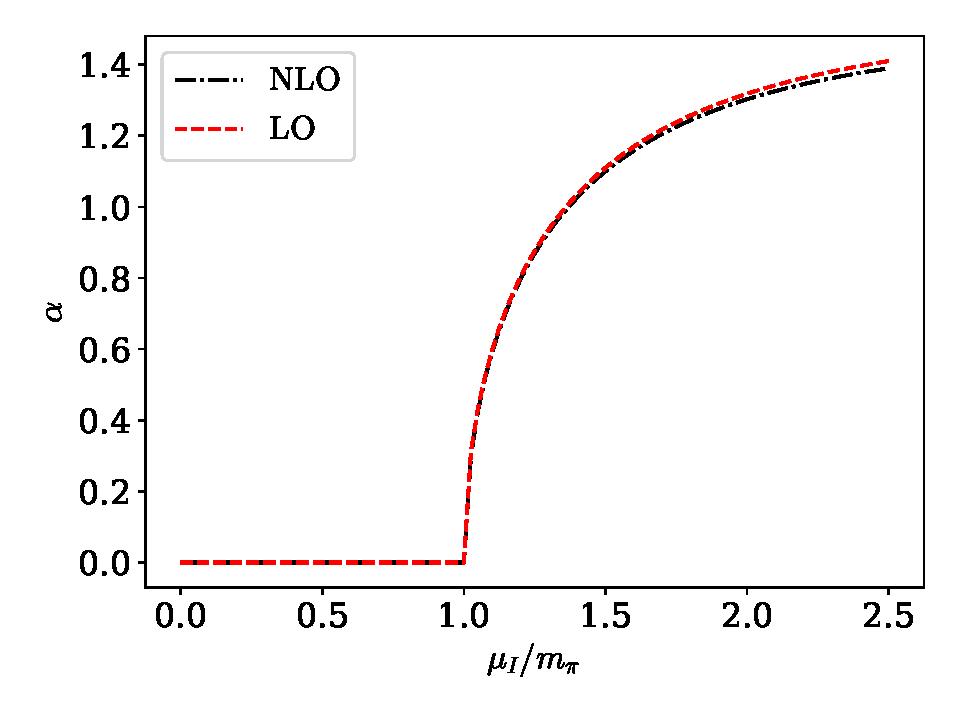
\includegraphics[width=0.7\textwidth]{figurer/numerics/alpha.pdf}
    \caption{The leading order and next-to-leading order results for $\alpha$ as a function of $\mu_I$.}
    \label{fig:alpha}
\end{figure}
